%-----------------------------------------------------------------------------------------------%
%
% Maret 2019
% Template Latex untuk Tugas Akhir Program Studi Sistem informasi ini
% dikembangkan oleh Inggih Permana (inggihjava@gmail.com)
%
% Template ini dikembangkan dari template yang dibuat oleh Andreas Febrian (Fasilkom UI 2003).
%
% Orang yang cerdas adalah orang yang paling banyak mengingat kematian.
%
%-----------------------------------------------------------------------------------------------%


%-----------------------------------------------------------------------------%
\chapter{\babEmpat}
\thispagestyle{fancy} % Menambahkan nomor halaman di ujung kanan
%-----------------------------------------------------------------------------%
\section{Analisis}
Analisis merupakan tahapan penting dalam pengembangan sistem yang melibatkan penguraian suatu pokok permasalahan menjadi bagian-bagian lebih kecil untuk dipelajari secara mendalam. Dalam konteks pengembangan sistem informasi, analisis bertujuan memahami kebutuhan pengguna, mengidentifikasi masalah yang ada pada sistem berjalan, serta merumuskan solusi tepat untuk mengatasi permasalahan tersebut. Proses analisis meliputi beberapa kegiatan utama, antara lain:
\begin{enumerate}
	\item Pengumpulan data dan informasi melalui observasi, wawancara, dan studi dokumentasi
	\item Identifikasi masalah pada sistem yang sedang berjalan
	\item Analisis kebutuhan fungsional dan non-fungsional sistem
	\item Evaluasi terhadap sistem yang ada untuk menemukan kekurangan dan peluang pengembangan
	\item Perumusan solusi dan rekomendasi untuk pengembangan sistem baru
\end{enumerate}

Pada bab ini, analisis dilakukan terhadap sistem yang berjalan di Laboratorium Program Studi Sistem Informasi, khususnya SITARIS, untuk mengidentifikasi kekurangan dan kebutuhan pengembangan lebih lanjut menjadi sistem manajemen laboratorium yang terintegrasi. Hasil analisis ini akan menjadi dasar dalam perancangan dan pengembangan sistem usulan.

\subsection{Analisis Sistem Berjalan}
Dalam proses tata kelola yang berlangsung di laboratorium Program Studi Sistem Informasi, hingga saat ini laboratorium telah menerapkan beberapa sistem informasi untuk mengelola berbagai aspek operasionalnya. Sistem-sistem tersebut meliputi:

\begin{enumerate}
	\item \textit{Laboratory Visitor Information System} disingkat LABVIS adalah sistem informasi yang digunakan untuk mengelola data kunjungan masuk dan keluar laboratorium, memungkinkan pemantauan dan pencatatan aktivitas pengunjung secara efisien seperti pada Lampiran \ref{fig:labvis-bab2}.

	\item \textit{Laboratory Assistant Registration Information System} disingkat LARIS adalah sistem informasi untuk mengelola data pendaftar dan proses rekrutmen asisten laboratorium seperti pada Lampiran \ref{fig:laris-bab2}.

	\item Sistem Informasi Inventaris disingkat SITARIS adalah sistem informasi inventarisasi yang memfasilitasi pengelolaan dan pemantauan alat serta barang di laboratorium, meningkatkan efisiensi dalam manajemen inventaris seperti pada Gambar \ref{fig:sitaris}.
\end{enumerate}

Implementasi sistem-sistem ini telah secara signifikan meningkatkan efektivitas dan efisiensi tata kelola laboratorium Program Studi Sistem Informasi, memungkinkan pengelolaan yang lebih terstruktur dan terintegrasi dalam berbagai aspek operasional laboratorium. Berdasarkan hasil observasi, ditemukan sejumlah permasalahan yang cukup krusial dalam sistem, antara lain kesalahan dalam pembuatan kode barang (Lampiran B), serta disfungsi pada fitur peminjaman barang dan ruangan (Lampiran B). Fitur peminjaman tersebut belum berjalan secara optimal dan belum sepenuhnya memenuhi Standar Operasional Prosedur (SOP) yang telah ditetapkan. Beberapa kelemahan yang teridentifikasi meliputi kurangnya akurasi dalam pencatatan data peminjaman, tidak adanya sistem verifikasi yang memadai untuk memastikan status barang atau ruangan yang dipinjam, serta minimnya notifikasi atau pelacakan terhadap barang yang masih berada dalam status dipinjam. Selain itu, sistem juga belum mampu secara otomatis mendeteksi dan memperbarui status barang yang telah dikembalikan, sehingga berpotensi menimbulkan kesalahan dalam inventarisasi. Kekurangan-kekurangan ini tidak hanya menghambat efisiensi operasional, tetapi juga berisiko menimbulkan kehilangan atau ketidaksesuaian data dalam manajemen aset secara keseluruhan, serta ketidaksesuaian format laporan akhir dengan kebutuhan kepala laboratorium (Lampiran B). Sistem tersebut masih memiliki kekurangan dalam menunjang tata kelola laboratorium, terutama dalam hal penjadwalan. Saat ini, tidak ada sistem informasi yang secara khusus mengelola penjadwalan laboratorium Program Studi Sistem Informasi. Pengelolaan penjadwalan masih dilakukan secara manual dengan melakukan validasi dan pengecekan pada jadwal yang diperoleh dari Ketua Program Studi. Keterbatasan ini berdampak signifikan pada efektivitas manajemen laboratorium secara keseluruhan dan mengakibatkan ketidaksesuaian dan kurangnya informasi mengenai jadwal praktikum di laboratorium. Oleh karena itu, perlu dilakukan penyempurnaan pada sistem informasi yang ada, khususnya SITARIS, agar dapat memenuhi kebutuhan tata kelola laboratorium dalam hal penjadwalan ruangan.

\subsection{Analisis Sistem Usulan}
Pengembangan sistem ini menyajikan fitur penjadwalan laboratorium yang dapat digunakan oleh Admin, Kaprodi, Sekprodi, dan Aslab. Fitur ini dirancang untuk mempermudah pengelolaan jadwal kegiatan di laboratorium, sehingga setiap pengguna dapat dengan mudah mengakses dan mengelola informasi terkait jadwal. Selain itu, sistem ini juga akan mengintegrasikan sistem informasi yang sudah ada seperti LABVIS, dan LARIS. Penyempurnaan ini bertujuan untuk mencapai tujuan laboratorium dalam menerapkan \textit{Integrated Laboratory Management Information System} (ILMIS) yang akan mengintegrasikan seluruh aspek manajemen laboratorium, termasuk penjadwalan, ke dalam satu sistem yang efisien. Dengan adanya sistem ini, diharapkan akan tercipta efisiensi dalam pengelolaan waktu dan sumber daya di laboratorium, serta mengurangi kemungkinan terjadinya bentrok jadwal antara berbagai kegiatan yang berlangsung dan juga mengintegrasikan sistem yang mulanya berdiri sendiri. Hasil akhir dari sistem ini adalah sebuah sistem terintegrasi yang memungkinkan semua pengguna untuk mengelola dan memantau jadwal laboratorium secara \textit{real-time}, meningkatkan koordinasi antar pengguna, dan memastikan bahwa semua kegiatan laboratorium dapat berjalan dengan lancar tanpa adanya konflik jadwal.

% \subsection{Analisis Kebutuhan Sistem}
\subsection{Analisis Kebutuhan Fungsional Sistem}
Sistem ini dirancang untuk memenuhi berbagai kebutuhan fungsional yang esensial dalam pengelolaan penjadwalan laboratorium. Sistem ini juga mendukung proses validasi yang terstruktur  untuk memantau dan memberitahukan status penggunaan laboratorium kepada pengguna. Pengelolaan akses pengguna yang aman dan integrasi yang lancar dengan sistem internal laboratorium lainnya juga menjadi bagian integral dari fungsi sistem ini, memastikan efisiensi dan transparansi dalam seluruh proses penjadwalan laboratorium.

\subsection{Analisis Kebutuhan Non-Fungsional Sistem}
Kebutuhan non-fungsional sistem terbagi dalam dua kategori utama yaitu kebutuhan perangkat lunak dan kebutuhan perangkat keras. Analisis terhadap kebutuhan perangkat keras dilakukan untuk mengoptimalkan dan mempermudah proses perancangan serta implementasi sistem yang akan dibangun.
% -----------------------------------------------------------------------------%
\begin{enumerate}
\item Analisis Kebutuhan Perangkat Lunak \\
Pada tahap analisis ini, peneliti mengidentifikasi dan mendefinisikan segala kebutuhan yang harus dipenuhi oleh sistem yang akan dikembangkan. Fokus utama dari analisis ini adalah memahami secara mendalam tujuan dan kebutuhan pengguna akhir, baik itu Admin, Kalab, Kaprodi, Sekprodi dan Aslab. Analisis kebutuhan perangkat lunak dapat dilihat pada Tabel \ref{tab:AnalisisKebutuhanPerangkatLunak}.

{
\fontsize{10}{13}\selectfont
\begin{longtable}{p{0.5cm} p{5cm} p{3cm} p{3.9cm}}
\caption{Analisis Kebutuhan Perangkat Lunak Pengembang}
\label{tab:AnalisisKebutuhanPerangkatLunak}                                                                                                 \\
\hline
\textbf{No} & \textbf{Perangkat Lunak}     & \textbf{Versi Minimal} & \textbf{Versi Tersedia}                                               \\ \hline
\endfirsthead

\multicolumn{4}{c}{\normalsize\tablename\ \textbf{\thetable}\ {{Analisis Kebutuhan Perangkat Lunak Pengembang \space (Tabel lanjutan...)}}} \\
\hline
\textbf{No} & \textbf{Perangkat Lunak}     & \textbf{Versi Minimal} & \textbf{Versi Tersedia}                                               \\ \hline
\endhead

\hline
\endfoot

1           & Windows                      & W8                     & W11                                                                   \\
2           & Balsamiq Mockup              & 4.0.0                  & 4.7.5                                                                 \\
3           & Google Chrome                & -                      & 127.0.6533.100                                                        \\
4           & MySQL                        & 8.0.0                  & 8.0.30                                                                \\
5           & VS Code                      & 1.71.1                 & 1.92.1                                                                \\
6           & Hypertext Preprocessor (PHP) & 8.0.0                  & 8.2.16                                                                \\
7           & CodeIgniter                  & 4                      & 4                                                                     \\
\hline
\end
{longtable}
}

\item Analisis Kebutuhan Perangkat Keras \\
Pada tahap analisis ini, peneliti mengidentifikasi dan mendefinisikan kebutuhan perangkat keras yang diperlukan dalam pengembangan sistem. Analisis ini bertujuan untuk memahami kebutuhan pengguna dan merancang solusi yang tepat dalam mengelola tata kelola laboratorium. Rincian analisis kebutuhan dapat dilihat pada Tabel \ref{tab:PerangkatKerasPengembang}.

{
\fontsize{10}{13}\selectfont
\begin{longtable}{p{0.5cm} p{5cm} p{2.4cm} p{3.9cm}}
\caption{Analisis Kebutuhan Perangkat Keras Pengembang}
\label{tab:PerangkatKerasPengembang}                                                                                                                                                                                                                                                            \\
\hline
\textbf{No} & \textbf{Perangkat Keras}     & \textbf{Versi Minimal} & \textbf{Versi Tersedia}                                               \\ \hline
\endfirsthead

\multicolumn{4}{c}{\normalsize\tablename\ \textbf{\thetable}\ {{Analisis Kebutuhan Perangkat Keras Pengembang \space (Tabel lanjutan...)}}} \\

\hline
\textbf{No} & \multicolumn{1}{c}{\textbf{Perangkat Keras}} & \multicolumn{1}{c}{\textbf{Spesifikasi Minimal}}                                                     & \multicolumn{1}{c}{\textbf{Versi Tersedia}}                                                                                 \\ \hline
\endhead

\hline
\endfoot


1           & \textit{Processor}                           & \begin{tabular}[c]{@{}l@{}}\textit{Intel Core i3} atau \\ \textit{AMD}  \textit{Ryzen} 3\end{tabular} & \begin{tabular}[c]{@{}l@{}}\textit{AMD Ryzen} 5 5600U, \\ 6 \textit{Cores}, 12 \textit{Threads}\end{tabular} \\
2           & \textit{Memory}                              & 4 \textit{GB DDR4}                                                                                   & 16 \textit{GB DDR4}-3200 \textit{MHz}                                                                                       \\
3           & \textit{Storage}                             & \begin{tabular}[c]{@{}l@{}}256 \textit{GB SSD} atau \\ 500 \textit{GB HDD}\end{tabular}              & 512 \textit{GB M.2 NVMe}                                                                                                    \\
4           & \textit{Keyboard}                            & \begin{tabular}[c]{@{}l@{}}\textit{Standard QWERTY} \\ \textit{keyboard}\end{tabular}                & 6-\textit{row}, \textit{multimedia Fn keys}                                                                                 \\
5           & \textit{Connection}                          & \begin{tabular}[c]{@{}l@{}}\textit{Wi-Fi} 802.11n atau \\ \textit{Ethernet}\end{tabular}             & \textit{Wi-Fi}® 6                                                                                                           \\
6           & \textit{Monitor}                             & \begin{tabular}[c]{@{}l@{}}14 \textit{inch}, resolusi \\ 1366x768\end{tabular}                       & 13 \textit{inc}                                                                                                             \\
\hline
\end
{longtable}
}

Dalam spesifikasi perangkat keras yang disarankan pada Sistem \textit{Integrated Laboratory Management Information System} sesuai yang tertera pada Tabel \ref{tab:PerangkatKerasPengembang} sebaiknya memenuhi syarat spesifikasi minimum agar sistem dapat berjalan dengan sempurna. Penggunaan perangkat keras dengan spesifikasi yang lebih tinggi dari minimum dapat meningkatkan performa sistem secara signifikan. Selain itu, pemilihan perangkat keras yang tepat juga akan mempengaruhi stabilitas dan keandalan sistem dalam jangka panjang.

\end{enumerate}

% =======================================================================================================================
\section{Perancangan}
Perancangan sistem perlu dilakukan sebelum dilakukan pembuatan sistem. tujuan dari perancangan sistem adalah untuk menentukan, mengorganisir, dan membentuk komponen dari solusi sistem akhir sehingga memiliki \textit{blueprint} untuk membangun sistem.

% =======================================================================================================================
\subsection{\textit{Use Case Diagram}}
\textit{\textit{Use Case} Diagram} terdiri dari \textit{actor}, \textit{use case} serta hubungannya. \textit{\textit{Use Case Diagram}} adalah sesuatu yang penting untuk memvisualisasiakan, menspesifikasikan dan mendokumentasikan kebutuhan perilaku sistem. \textit{\textit{Use Case Diagram}} digunakan untuk menjelaskan kegiatan apa saja yang dapat dilakukan oleh \textit{user} pengguna sistem yang sedang berjalan \cite{Carstoiu1995}. Dalam pengembangan sistem manajemen laboratorium ini, \textit{Use Case Diagram} membantu mengidentifikasi interaksi antara pengguna dengan sistem secara jelas. Setiap aktor dalam diagram memiliki peran dan hak akses yang berbeda sesuai dengan kebutuhan fungsional sistem. Dengan adanya \textit{Use Case Diagram}, tim pengembang dapat memahami alur kerja sistem dari perspektif pengguna. Selain itu, diagram ini juga berfungsi sebagai dasar komunikasi antara pengembang dan pemangku kepentingan untuk memastikan bahwa sistem yang dibangun sesuai dengan kebutuhan.

	{
		\fontsize{10}{13}\selectfont
		\begin{longtable}{p{0.5cm} p{3cm} p{9.3cm}}
			\caption{Deskripsi Aktor}
			\label{tab:DeskripsiAktor}                                                                                    \\
			\hline
			\textbf{No} & \textbf{Aktor} & \textbf{Deskripsi}                                                             \\ \hline
			\endfirsthead

			\multicolumn{3}{c}{\normalsize\tablename\ \textbf{\thetable}\ {{Deskripsi Aktor \space (Tabel lanjutan...)}}} \\
			\hline
			\textbf{No} & \textbf{Aktor} & \textbf{Deskripsi}                                                             \\ \hline
			\endhead

			\hline
			\endfoot

			1           & Admin          & Mengelola penjadwalan laboratorium termasuk lihat, tambah, edit, dan hapus     \\
			2           & Kalab          & Mengelola penjadwalan laboratorium termasuk lihat, tambah, edit, dan hapus     \\
			3           & Kaprodi        & Melihat penjadwalan laboratorium                                               \\
			4           & Sekprodi       & Melihat penjadwalan laboratorium                                               \\
			5           & Aslab          & Mengelola penjadwalan laboratorium termasuk lihat, tambah, edit, dan hapus     \\ \hline
		\end{longtable}
	}

Sistem manajemen laboratorium adalah sistem yang dikelola secara terpusat oleh seorang Admin. Sistem ini digambarkan menggunakan diagram \textit{use case} yang menunjukkan interaksi antara admin dengan berbagai komponen sistem. Dalam sistem ini terdapat 4 fungsi utama yang dapat digunakan oleh admin dalam mengelola sistem. Fungsi-fungsi tersebut meliputi kemampuan Admin untuk menambahkan jadwal baru melalui menu "Tambah Jadwal Laboratorium", mengubah jadwal yang ada melalui "Edit Jadwal Laboratorium", menghapus jadwal yang tidak diperlukan melalui "Hapus Jadwal Laboratorium", dan melihat daftar jadwal melalui "Lihat Jadwal Laboratorium".

Keamanan sistem dijamin melalui mekanisme \textit{login} yang ditunjukkan dengan relasi \textit{"include"} pada diagram. Tiga fungsi utama yaitu penambahan, pengeditan, dan penghapusan jadwal termasuk ke dalam lingkup wewenang Admin, oleh karena itu fungsi-fungsi tersebut mengharuskan Admin untuk \textit{login} terlebih dahulu sebelum dapat mengaksesnya. Sementara itu, fungsi melihat jadwal laboratorium dapat diakses langsung tanpa memerlukan \textit{login} seperti yang ditunjukkan dalam Gambar \ref{usecase-diagram-admin}.

\begin{figure}
	\centering
	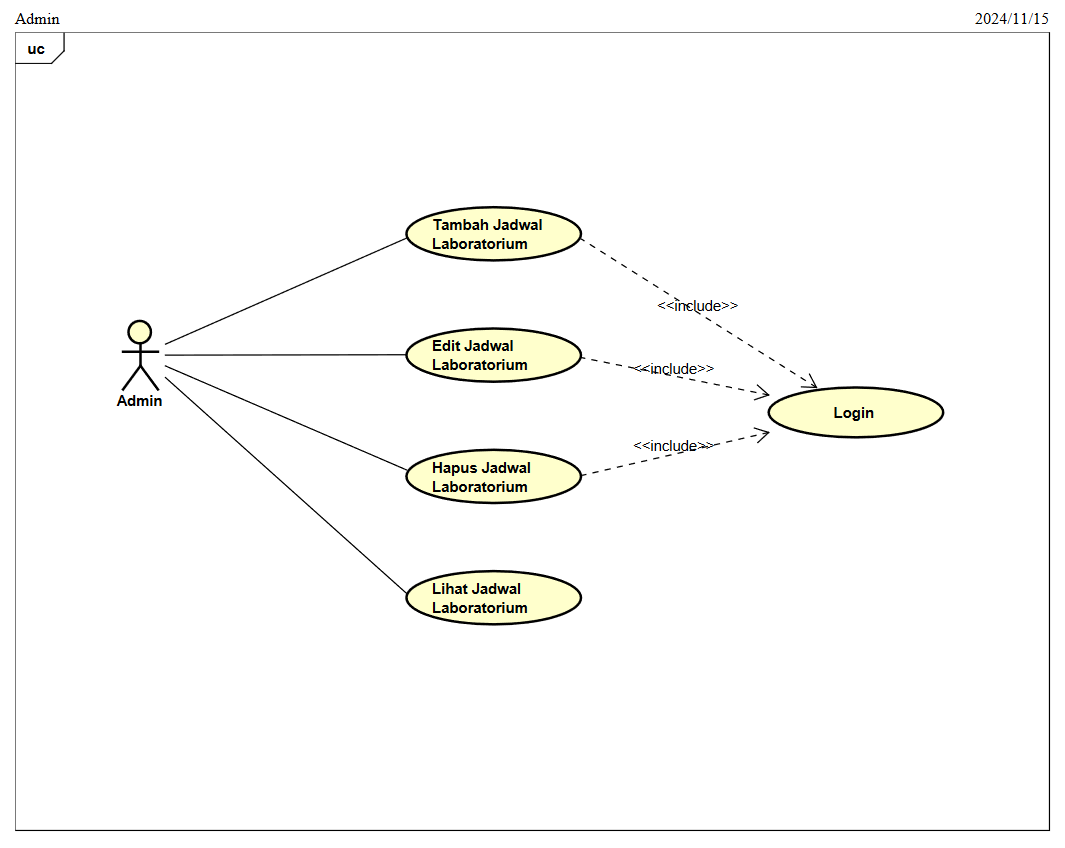
\includegraphics[width=1\textwidth]{konten/gambar/usecase-diagram/admin.png}
	\caption{\textit{Use Case Diagram} Admin}
	\label{usecase-diagram-admin}
\end{figure}

Dalam sistem ini, Kalab memiliki empat fungsi utama yang dapat diakses. Fungsi-fungsi tersebut meliputi kemampuan untuk menambahkan jadwal baru melalui fitur "Tambah Jadwal Laboratorium", melakukan perubahan pada jadwal yang sudah ada menggunakan fitur "Edit Jadwal Laboratorium", menghapus jadwal yang tidak diperlukan dengan fitur "Hapus Jadwal Laboratorium", dan melihat seluruh daftar jadwal yang tersedia melalui fitur "Lihat Jadwal Laboratorium". Keamanan sistem dijamin melalui mekanisme \textit{login} yang ditunjukkan dengan relasi \textit{"include"} pada diagram. Tiga fungsi utama, yaitu menambah, mengedit, dan menghapus jadwal, mengharuskan Kalab untuk melakukan \textit{login} terlebih dahulu sebelum dapat mengakses fungsi-fungsi tersebut. Sementara itu, fungsi untuk melihat jadwal laboratorium dapat diakses secara langsung tanpa perlu melalui proses \textit{login} terlebih dahulu, seperti yang ditunjukkan pada Lampiran \ref{usecase-diagram-kalab}.

Dalam sistem ini, Kaprodi memiliki satu fungsi utama yang dapat diakses, yaitu melihat seluruh daftar jadwal yang tersedia melalui fitur "Lihat Jadwal Laboratorium". Fungsi ini dapat diakses secara langsung tanpa perlu melalui proses \textit{login} terlebih dahulu, sehingga Kaprodi dapat dengan mudah memantau jadwal laboratorium yang ada. Hal ini ditunjukkan pada Lampiran \ref{usecase-diagram-kaprodi}.

Dalam sistem ini, Sekprodi memiliki satu fungsi utama yang dapat diakses, yaitu melihat seluruh daftar jadwal yang tersedia melalui fitur "Lihat Jadwal Laboratorium". Fungsi ini dapat diakses secara langsung tanpa perlu melalui proses \textit{login} terlebih dahulu, sehingga Sekprodi dapat dengan mudah memantau jadwal laboratorium yang ada. Hal ini ditunjukkan pada Lampiran \ref{usecase-diagram-sekprodi}.

Dalam sistem ini, Aslab memiliki empat fungsi utama yang dapat diakses. Fungsi-fungsi tersebut meliputi kemampuan untuk menambahkan jadwal baru melalui fitur "Tambah Jadwal Laboratorium", melakukan perubahan pada jadwal yang sudah ada menggunakan fitur "Edit Jadwal Laboratorium", menghapus jadwal yang tidak diperlukan dengan fitur "Hapus Jadwal Laboratorium", dan melihat seluruh daftar jadwal yang tersedia melalui fitur "Lihat Jadwal Laboratorium". Keamanan sistem dijamin melalui mekanisme \textit{login} yang ditunjukkan dengan relasi "include" pada diagram. Tiga fungsi utama, yaitu menambah, mengedit, dan menghapus jadwal, mengharuskan Aslab untuk melakukan \textit{login} terlebih dahulu sebelum dapat mengakses fungsi-fungsi tersebut. Sementara itu, fungsi untuk melihat jadwal laboratorium dapat diakses secara langsung tanpa perlu melalui proses \textit{login} terlebih dahulu, seperti yang ditunjukkan pada Lampiran \ref{usecase-diagram-aslab}.

% Skenario \textit{use case Login} merujuk pada rangkaian langkah-langkah terstruktur yang harus dilakukan oleh pengguna untuk melakukan proses kegiatan dalam suatu sistem. Proses ini dimulai dengan pengguna yang ingin mengakses sistem harus memasukkan informasi identifikasi pribadi, seperti nim, dan kata sandi, guna memverifikasi identitas mereka. Setelah pengisian data, sistem akan melakukan verifikasi dengan data yang tercatat dalam basis data, dan jika sesuai, pengguna akan diberikan izin akses ke fitur atau informasi yang relevan. Skenario \textit{Use Case Login} memegang peran krusial dalam menjaga tingkat keamanan serta privasi sistem, menjamin bahwa hanya pengguna yang diberi akses yang dapat masuk kedalam sistem.

% Pentingnya tahap ini dalam keamanan sistem ditunjukkan dalam Tabel \ref{tab:SkenarioLogin} yang secara rinci menggambarkan langkah-langkah dalam proses otentikasi. Dengan menjamin kelancaran proses ini, sistem dapat melindungi data sensitif dan memastikan bahwa hanya pengguna yang berwenang yang memiliki akses ke informasi yang terdapat dalam sistem.

% 	{
% 		\fontsize{10}{12}
% 		\begin{longtable}{@{} p{6cm} p{6cm} @{}}
% 			\caption{Skenario \textit{Use Case Login}} \label{tab:SkenarioLogin}                                                                                                                                                                                                           \\ \hline
% 			\textbf{Nama use case}                                                                         & \textit{Login}                                                                                                                                                                \\
% 			\textbf{Aktor}                                                                                 & Admin, Kalab, Aslab, Pendaftar.                                                                                                                                               \\
% 			\textbf{Deskripsi}                                                                             & \textit{Use case} ini menggambarkan untuk dapat mengelola sistem, Admin, Kepala Laboratorium, Pendaftar, Asisten Laboratorium harus melakukan \textit{login} terlebih dahulu. \\
% 			\textbf{Kondisi Awal}                                                                          & Sistem menampilkan form \textit{login}.                                                                                                                                       \\
% 			\textbf{Kondisi Akhir}                                                                         & Sistem menampilkan menu utama.                                                                                                                                                \\ \hline
% 			\multicolumn{1}{c}{\textbf{Aktor}}                                                             & \multicolumn{1}{c}{\textbf{Sistem}}                                                                                                                                           \\ \hline
% 			\multicolumn{2}{c}{\textbf{Skenario normal}}                                                                                                                                                                                                                                   \\ \hline
% 			1. \textit{Use case} ini dimulai ketika Admin, Kalab, Kaprodi, Sekprodi, Aslab \textit{login}. &                                                                                                                                                                               \\
% 			                                                                                               & 2. Sistem melakukan verifikasi \textit{login}.                                                                                                                                \\
% 			                                                                                               & 3. Sistem menampilkan menu utama.                                                                                                                                             \\ \hline
% 			\multicolumn{2}{c}{\textbf{Skenario gagal}}                                                                                                                                                                                                                                    \\ \hline
% 			1. \textit{Use case} ini dimulai ketika Admin, Kalab, Kaprodi, Sekprodi, Aslab \textit{login}. &                                                                                                                                                                               \\
% 			                                                                                               & 2. Sistem melakukan verifikasi \textit{login}.                                                                                                                                \\
% 			                                                                                               & 3. Sistem menampilkan pesan \textit{login} tidak valid.                                                                                                                       \\ \hline
% 		\end{longtable}}

% 	{
% 		\fontsize{10}{12}
% 		\begin{longtable}{@{} p{6cm} p{6cm} @{}}
% 			\caption{Skenario \textit{Use Case Kalab}} \label{tab:SkenarioKalab}                                                                                                                                             \\ \hline
% 			\textbf{Nama use case}                            & \textit{Manajemen Jadwal Laboratorium}                                                                                                                       \\
% 			\textbf{Aktor}                                    & Kalab, Aslab.                                                                                                                                                \\
% 			\textbf{Deskripsi}                                & \textit{Use case} ini menggambarkan proses yang dilakukan oleh Kalab untuk mengelola jadwal laboratorium, termasuk menambah, mengedit, dan menghapus jadwal. \\
% 			\textbf{Kondisi Awal}                             & Sistem menampilkan menu manajemen jadwal.                                                                                                                    \\
% 			\textbf{Kondisi Akhir}                            & Sistem menampilkan daftar jadwal laboratorium yang telah diperbarui.                                                                                         \\ \hline
% 			\multicolumn{1}{c}{\textbf{Aktor}}                & \multicolumn{1}{c}{\textbf{Sistem}}                                                                                                                          \\ \hline
% 			\multicolumn{2}{c}{\textbf{Skenario normal}}                                                                                                                                                                     \\ \hline
% 			1. Kalab memilih opsi untuk menambah jadwal baru. &                                                                                                                                                              \\
% 			                                                  & 2. Sistem menampilkan form untuk input jadwal baru.                                                                                                          \\
% 			                                                  & 3. Kalab mengisi form dan mengirimkan data.                                                                                                                  \\
% 			                                                  & 4. Sistem menyimpan jadwal baru dan menampilkan konfirmasi.                                                                                                  \\ \hline
% 			\multicolumn{2}{c}{\textbf{Skenario gagal}}                                                                                                                                                                      \\ \hline
% 			1. Kalab memilih opsi untuk menambah jadwal baru. &                                                                                                                                                              \\
% 			                                                  & 2. Sistem menampilkan form untuk input jadwal baru.                                                                                                          \\
% 			                                                  & 3. Kalab mengisi form dengan data yang tidak valid.                                                                                                          \\
% 			                                                  & 4. Sistem menampilkan pesan kesalahan dan meminta Kalab untuk memperbaiki data.                                                                              \\ \hline
% 		\end{longtable}}
% 	{

% 		\fontsize{10}{12}
% 		\begin{longtable}{@{} p{6cm} p{6cm} @{}}
% 			\caption{Skenario \textit{Use Case Kalab}} \label{tab:SkenarioKalab}                                                                                                                                             \\ \hline
% 			\textbf{Nama use case}                            & \textit{Manajemen Jadwal Laboratorium}                                                                                                                       \\
% 			\textbf{Aktor}                                    & Kalab, Aslab.                                                                                                                                                \\
% 			\textbf{Deskripsi}                                & \textit{Use case} ini menggambarkan proses yang dilakukan oleh Kalab untuk mengelola jadwal laboratorium, termasuk menambah, mengedit, dan menghapus jadwal. \\
% 			\textbf{Kondisi Awal}                             & Sistem menampilkan menu manajemen jadwal.                                                                                                                    \\
% 			\textbf{Kondisi Akhir}                            & Sistem menampilkan daftar jadwal laboratorium yang telah diperbarui.                                                                                         \\ \hline
% 			\multicolumn{1}{c}{\textbf{Aktor}}                & \multicolumn{1}{c}{\textbf{Sistem}}                                                                                                                          \\ \hline
% 			\multicolumn{2}{c}{\textbf{Skenario normal}}                                                                                                                                                                     \\ \hline
% 			1. Kalab memilih opsi untuk menambah jadwal baru. &                                                                                                                                                              \\
% 			                                                  & 2. Sistem menampilkan form untuk input jadwal baru.                                                                                                          \\
% 			                                                  & 3. Kalab mengisi form dan mengirimkan data.                                                                                                                  \\
% 			                                                  & 4. Sistem menyimpan jadwal baru dan menampilkan konfirmasi.                                                                                                  \\ \hline
% 			\multicolumn{2}{c}{\textbf{Skenario gagal}}                                                                                                                                                                      \\ \hline
% 			1. Kalab memilih opsi untuk menambah jadwal baru. &                                                                                                                                                              \\
% 			                                                  & 2. Sistem menampilkan form untuk input jadwal baru.                                                                                                          \\
% 			                                                  & 3. Kalab mengisi form dengan data yang tidak valid.                                                                                                          \\
% 			                                                  & 4. Sistem menampilkan pesan kesalahan dan meminta Kalab untuk memperbaiki data.                                                                              \\ \hline
% 		\end{longtable}}

% =======================================================================================================================
\subsection{\textit{Activity Diagram}}
\textit{Activity Diagram} adalah salah satu alat dalam \textit{Unified Modeling Language} (UML) yang digunakan untuk memvisualisasikan alur kerja atau aktivitas dalam suatu sistem \cite{linzhang2004generating}. Pada sistem ini, \textit{Activity Diagram} memberikan gambaran rinci tentang proses yang dilalui oleh berbagai aktor seperti Admin, Kalab, Kaprodi, Sekprodi, Aslab.

\textit{Activity Diagram} \textit{login} memberikan gambaran rinci tentang proses \textit{login} yang dilalui oleh pengguna. Diagram ini memandu langkah-langkah yang terlibat dalam proses \textit{login}, mulai dari input data oleh pengguna, validasi oleh sistem hingga dapat masuk ke dalam sistem menggunakan akun yang sudah ada. \textit{Activity Diagram} ini dapat dilihat pada Gambar \ref{activity-diagram-login}.

\begin{figure}
	\centering
	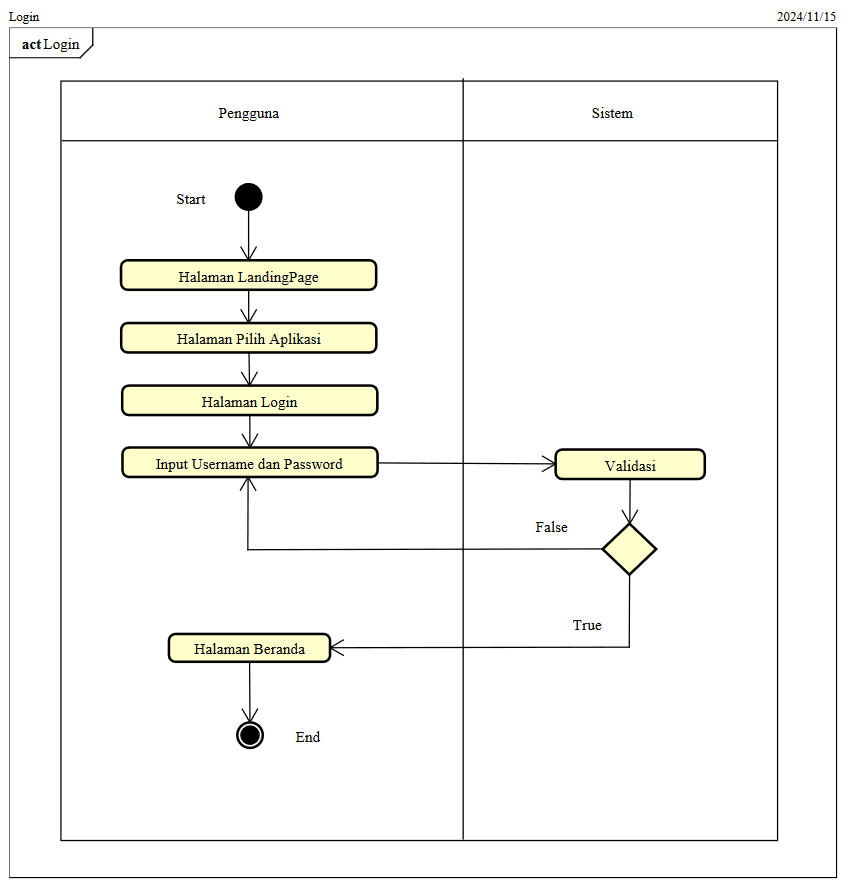
\includegraphics[width=1\textwidth]{konten/gambar/activity-diagram/login.png}
	\caption{\textit{Activity Diagram Login}}
	\label{activity-diagram-login}
\end{figure}

\textit{Activity Diagram} tambah dosen memberikan gambaran rinci tentang proses penambahan dosen yang dilalui oleh pengguna. Diagram ini memandu langkah-langkah yang terlibat dalam proses penambahan dosen, mulai dari input data oleh pengguna, validasi oleh sistem hingga penyimpanan data dosen baru ke dalam sistem. \textit{Activity Diagram} ini dapat dilihat pada Lampiran \ref{activity-diagram-tambah-dosen}.

\textit{Activity Diagram} edit dosen memberikan gambaran rinci tentang proses pengeditan data dosen yang dilalui oleh pengguna. Diagram ini memandu langkah-langkah yang terlibat dalam proses pengeditan dosen, mulai dari pemilihan data dosen yang akan diedit, input data baru oleh pengguna, validasi oleh sistem hingga penyimpanan data dosen yang telah diperbarui ke dalam sistem. \textit{Activity Diagram} ini dapat dilihat pada Lampiran \ref{activity-diagram-edit-dosen}.

\textit{Activity Diagram} hapus dosen memberikan gambaran rinci tentang proses penghapusan dosen yang dilalui oleh pengguna. Diagram ini memandu langkah-langkah yang terlibat dalam proses penghapusan dosen, mulai dari pemilihan data dosen yang akan dihapus, konfirmasi oleh pengguna, hingga penghapusan data dosen dari sistem. \textit{Activity Diagram} ini dapat dilihat pada Lampiran \ref{activity-diagram-hapus-dosen}.


\textit{Activity Diagram} tambah mata kuliah memberikan gambaran rinci tentang proses penambahan mata kuliah yang dilalui oleh pengguna. Diagram ini memandu langkah-langkah yang terlibat dalam proses penambahan mata kuliah, mulai dari input data oleh pengguna, validasi oleh sistem hingga penyimpanan data mata kuliah baru ke dalam sistem. \textit{Activity Diagram} ini dapat dilihat pada Lampiran \ref{activity-diagram-tambah-matkul}.


\textit{Activity Diagram} edit mata kuliah memberikan gambaran rinci tentang proses pengeditan data mata kuliah yang dilalui oleh pengguna. Diagram ini memandu langkah-langkah yang terlibat dalam proses pengeditan mata kuliah, mulai dari pemilihan data mata kuliah yang akan diedit, input data baru oleh pengguna, validasi oleh sistem hingga penyimpanan data mata kuliah yang telah diperbarui ke dalam sistem. \textit{Activity Diagram} ini dapat dilihat pada Lampiran \ref{activity-diagram-edit-matkul}.


\textit{Activity Diagram} hapus mata kuliah memberikan gambaran rinci tentang proses penghapusan mata kuliah yang dilalui oleh pengguna. Diagram ini memandu langkah-langkah yang terlibat dalam proses penghapusan mata kuliah, mulai dari pemilihan data mata kuliah yang akan dihapus, konfirmasi oleh pengguna, hingga penghapusan data mata kuliah dari sistem. \textit{Activity Diagram} ini dapat dilihat pada Lampiran \ref{activity-diagram-hapus-matkul}.


\textit{Activity Diagram} tambah jadwal memberikan gambaran rinci tentang proses penambahan jadwal yang dilalui oleh pengguna. Diagram ini memandu langkah-langkah yang terlibat dalam proses penambahan jadwal, mulai dari input data oleh pengguna, validasi oleh sistem hingga penyimpanan data jadwal baru ke dalam sistem. \textit{Activity Diagram} ini dapat dilihat pada Lampiran \ref{activity-diagram-tambah-jadwal}.


\textit{Activity Diagram} edit jadwal memberikan gambaran rinci tentang proses pengeditan jadwal yang dilalui oleh pengguna. Diagram ini memandu langkah-langkah yang terlibat dalam proses pengeditan jadwal, mulai dari pemilihan data jadwal yang akan diedit, input data baru oleh pengguna, validasi oleh sistem hingga penyimpanan data jadwal yang telah diperbarui ke dalam sistem. \textit{Activity Diagram} ini dapat dilihat pada Lampiran \ref{activity-diagram-edit-jadwal}.


\textit{Activity Diagram} hapus jadwal memberikan gambaran rinci tentang proses penghapusan jadwal yang dilalui oleh pengguna. Diagram ini memandu langkah-langkah yang terlibat dalam proses penghapusan jadwal, mulai dari pemilihan data jadwal yang akan dihapus, konfirmasi oleh pengguna, hingga penghapusan data jadwal dari sistem. \textit{Activity Diagram} ini dapat dilihat pada Lampiran \ref{activity-diagram-hapus-jadwal}.


% =======================================================================================================================
\subsection{\textit{Class Diagram}}
\textit{Class Diagram} adalah representasi visual dari struktur kelas dalam sistem manajemen laboratorium, yang menunjukkan hubungan logis antar kelas. \textit{Class Diagram} ini menyediakan deskripsi terperinci dari setiap kelas yang terlibat dalam sistem, termasuk atribut dan operasi yang diperlukan untuk mendukung fungsi manajemen laboratorium secara efektif. \textit{Class Diagram} Sistem Informasi Manajemen Laboratorium dapat dilihat pada Lampiran \ref{class-diagram}.

Relasi antara jadwal dengan ruangan, dosen, dan mata kuliah diwakili oleh id\_ruangan, id\_dosen, dan id\_matkul pada jadwal. Id\_ruangan menunjukkan keterkaitan jadwal dengan ruangan tertentu, id\_dosen menunjukkan keterkaitan jadwal dengan dosen tertentu, dan id\_matkul menunjukkan keterkaitan jadwal dengan mata kuliah tertentu. Hubungan ini digambarkan dengan garis yang menghubungkan entitas jadwal ke masing-masing entitas ruangan, dosen, dan mata kuliah dalam diagram.

% =======================================================================================================================
\subsection{Perancangan \textit{Database}}
Perancangan \textit{database} adalah perancangan basis data yang akan digunakan pada sebuah sistem, didasari oleh data perusahaan. Perancangan ini bertujuan agar tiap \texttt{field} data yang memiliki relasi dapat terhubung pada tabel di \textit{database}, sehingga proses pengaksesan data akan dapat telaksana dengan lebih baik. Berikut adalah detail perancangan serta relasi yang ada pada \textit{database} sistem informasi inventaris laboratorium pada Laboratorium Sistem Informasi. Berikut tabel perancangan \textit{database}:

\begin{enumerate}

	\item Perancangan \textit{Database} Tabel Dosen

	      Tabel Dosen dirancang untuk menyimpan informasi komprehensif tentang staf pengajar. Struktur tabel ini mencakup berbagai atribut yang diperlukan untuk mengidentifikasi dan mengelola data dosen secara efisien. Berikut adalah penjelasan ilmiah mengenai struktur dan fungsi Tabel Dosen:

	      \begin{enumerate}[label=\alph*.]
		      \item Tabel ini menetapkan \texttt{id\_dosen} sebagai kunci utama dengan tipe data \texttt{tinyint(4)} dan fitur \texttt{auto increment} yang memastikan bahwa setiap dosen diberikan identifikasi yang unik dalam sistem.
		      \item Atribut \texttt{'nama\_dosen'} dan \texttt{'nip\_dosen'} berfungsi untuk menyimpan informasi dasar tentang dosen yang memudahkan pengenalan personal dalam lingkungan akademis.
		      \item Atribut \texttt{'jenis\_kelamin'} memakai tipe data \texttt{enum} untuk menjaga konsistensi data dan membantu dalam analisis demografis.
		      \item \texttt{'email\_dosen'} dan \texttt{'no\_hp'} merupakan saluran komunikasi yang vital, memungkinkan komunikasi yang efektif antara dosen dan sistem.
		      \item Atribut \texttt{'nidn'} mencatat identifikasi nasional yang unik untuk dosen yang mendukung integrasi dengan sistem pendidikan tinggi yang lebih luas.
	      \end{enumerate}

	      Struktur tabel ini dirancang dengan mempertimbangkan kebutuhan manajemen data dosen yang komprehensif, efisiensi penyimpanan, dan kemudahan dalam pemrosesan dan analisis data.

		      {
			      \fontsize{10}{13}\selectfont
			      \begin{longtable}{p{3 cm} p{3cm} p{3 cm} p{3.4 cm}}
				      \caption{Perancangan Tabel Dosen}
				      \label{admin}                                                                                                                 \\
				      \hline
				      \textbf{\textit{Field}} & \textbf{\textit{Type}} & \textbf{\textit{Length}}            & \textbf{\textit{Key}}                \\
				      \hline
				      \endfirsthead

				      \multicolumn{4}{c}{\tablename\ \thetable\ {Perancangan Tabel Dosen} \space (Tabel lanjutan...)}                               \\
				      \hline
				      \textbf{\textit{Field}} & \textbf{\textit{Type}} & \textbf{\textit{Length}}            & \textbf{\textit{Key}}                \\
				      \hline
				      \endhead

				      \texttt{id\_dosen}      & \texttt{tinyint}       & \texttt{4}                          & \textit{\texttt{Primary key} (A\_I)} \\
				      \texttt{nama\_dosen}    & \texttt{varchar}       & \texttt{100}                        &                                      \\
				      \texttt{nip\_dosen}     & \texttt{varchar}       & \texttt{50}                         &                                      \\
				      \texttt{jenis\_kelamin} & \texttt{enum}          & \texttt{('Laki-laki', 'Perempuan')} &                                      \\
				      \texttt{email\_dosen}   & \texttt{varchar}       & \texttt{100}                        &                                      \\
				      \texttt{nidn}           & \texttt{varchar}       & \texttt{100}                        &                                      \\
				      \texttt{no\_hp}         & \texttt{varchar}       & \texttt{100}                        &                                      \\
				      \hline
			      \end{longtable}
		      }

	\item Perancangan \textit{Database} Tabel Matkul
	      Tabel Matkul dirancang untuk menyimpan informasi tentang mata kuliah yang ditawarkan dalam program akademik. Struktur tabel ini mencakup berbagai atribut yang diperlukan untuk mengidentifikasi dan mengelola data mata kuliah secara efisien. Berikut adalah penjelasan ilmiah mengenai struktur dan fungsi Tabel Matkul:

	      \begin{enumerate}[label=\alph*.]
		      \item Tabel ini memanfaatkan \texttt{id\_matkul} sebagai kunci utama dengan tipe data \texttt{tinyint(4)} dan fitur \texttt{auto increment}, yang menjamin bahwa setiap mata kuliah diberi identifikasi yang unik di dalam sistem.
		      \item Atribut \texttt{'kode\_matkul'} dan \texttt{'nama\_matkul'} berfungsi untuk menyimpan informasi dasar yang membantu dalam mengenali mata kuliah dengan cepat di lingkungan akademik.
		      \item Atribut \texttt{'sks'} dan \texttt{'semester'} berisi informasi krusial mengenai bobot akademik dan penjadwalan mata kuliah dalam kurikulum, yang penting untuk perencanaan pendidikan.
		      \item Atribut \texttt{'jenis\_matkul'} memakai tipe data \texttt{enum} untuk membedakan mata kuliah menjadi kategori wajib atau pilihan, mendukung kelancaran dalam pengelolaan kurikulum.
	      \end{enumerate}

	      Struktur tabel ini dirancang dengan mempertimbangkan kebutuhan manajemen data mata kuliah yang komprehensif, efisiensi penyimpanan, dan kemudahan dalam pemrosesan dan analisis data kurikulum.

		      {
			      \fontsize{10}{13}\selectfont
			      \begin{longtable}{p{3 cm} p{3cm} p{3 cm} p{3.4 cm}}
				      \caption{Perancangan Tabel Matkul}
				      \label{admin}                                                                                                           \\
				      \hline
				      \textbf{\textit{Field}} & \textbf{\textit{Type}} & \textbf{\textit{Length}}      & \textbf{\textit{Key}}                \\
				      \hline
				      \endfirsthead

				      \multicolumn{4}{c}{\tablename\ \thetable\ {Perancangan Tabel Matkul} \space (Tabel lanjutan...)}                        \\
				      \hline
				      \textbf{\textit{Field}} & \textbf{\textit{Type}} & \textbf{\textit{Length}}      & \textbf{\textit{Key}}                \\
				      \hline
				      \endhead

				      \texttt{id\_matkul}     & \texttt{tinyint}       & \texttt{4}                    & \textit{\texttt{Primary key} (A\_I)} \\
				      \texttt{kode\_matkul}   & \texttt{varchar}       & \texttt{50}                   &                                      \\
				      \texttt{nama\_matkul}   & \texttt{varchar}       & \texttt{100}                  &                                      \\
				      \texttt{sks}            & \texttt{tinyint}       & \texttt{4}                    &                                      \\
				      \texttt{semester}       & \texttt{tinyint}       & \texttt{4}                    &                                      \\
				      \texttt{jenis\_matkul}  & \texttt{enum}          & \texttt{('Wajib', 'Pilihan')} &                                      \\
				      \hline
			      \end{longtable}
		      }

	\item Perancangan \textit{Database} Tabel Ruangan

	      Tabel Ruangan dirancang untuk menyimpan informasi tentang ruangan-ruangan yang tersedia untuk kegiatan akademik. Struktur tabel ini mencakup berbagai atribut yang diperlukan untuk mengidentifikasi dan mengelola data ruangan secara efisien. Berikut adalah penjelasan ilmiah mengenai struktur dan fungsi Tabel Ruangan:

	      \begin{enumerate}[label=\alph*.]
		      \item Tabel ini memanfaatkan \texttt{id\_ruangan} sebagai \texttt{primary key}. Dengan menggunakan tipe data \texttt{tinyint(4)} dan fitur \texttt{auto increment}, tabel ini memastikan bahwa setiap ruangan tercatat dengan identitas uniknya sendiri dalam sistem.
		      \item Atribut \texttt{'id\_gedung'} bertindak sebagai \texttt{foreign key} yang mengaitkan setiap ruangan dengan gedungnya, membantu dalam mengatur lokasi dengan lebih terstruktur.
		      \item Atribut \texttt{'nama\_ruangan'} berisi nama yang memudahkan pengguna dalam mengenali setiap ruangan.
		      \item Atribut \texttt{'deskripsi\_ruangan'} memberikan ruang untuk menambahkan keterangan lebih lanjut mengenai fasilitas atau ciri khas dari ruangan tersebut.
		      \item Atribut \texttt{'gambar\_ruangan'} berisi jalur ke file gambar yang berkaitan dengan ruangan, memudahkan dalam visualisasi dan lebih memahami penampilan ruangan tersebut.
	      \end{enumerate}

	      Struktur tabel ini dirancang dengan mempertimbangkan kebutuhan manajemen data ruangan yang komprehensif, efisiensi penyimpanan, dan kemudahan dalam pemrosesan dan analisis data fasilitas.

		      {
			      \fontsize{10}{13}\selectfont
			      \begin{longtable}{p{3 cm} p{3cm} p{3 cm} p{3.4 cm}}
				      \caption{Perancangan Tabel Ruangan}
				      \label{admin}                                                                                                          \\
				      \hline
				      \textbf{\textit{Field}}     & \textbf{\textit{Type}} & \textbf{\textit{Length}} & \textbf{\textit{Key}}                \\
				      \hline
				      \endfirsthead

				      \multicolumn{4}{c}{\tablename\ \thetable\ {Perancangan Tabel Ruangan} \space (Tabel lanjutan...)}                      \\
				      \hline
				      \textbf{\textit{Field}}     & \textbf{\textit{Type}} & \textbf{\textit{Length}} & \textbf{\textit{Key}}                \\
				      \
				      \endhead

				      \texttt{id\_ruangan}        & \texttt{tinyint}       & \texttt{4}               & \textit{\texttt{Primary key} (A\_I)} \\
				      \texttt{id\_gedung}         & \texttt{tinyint}       & \texttt{4}               & \textit{\texttt{Foreign key}}        \\
				      \texttt{nama\_ruangan}      & \texttt{varchar}       & \texttt{100}             &                                      \\
				      \texttt{deskripsi\_ruangan} & \texttt{text}          &                          &                                      \\
				      \texttt{gambar\_ruangan}    & \texttt{varchar}       & \texttt{255}             &                                      \\
				      \hline
			      \end{longtable}
		      }

	\item Perancangan \textit{Database} Tabel Jadwal

	      Tabel Jadwal dirancang untuk menyimpan informasi tentang penjadwalan kegiatan akademik. Struktur tabel ini mencakup berbagai atribut yang diperlukan untuk mengidentifikasi dan mengelola data jadwal secara efisien. Berikut adalah penjelasan ilmiah mengenai struktur dan fungsi Tabel Jadwal:

	      \begin{enumerate}[label=\alph*.]
		      \item Tabel ini dilengkapi dengan \texttt{id\_jadwal} sebagai \texttt{primary key}. Dengan tipe data \texttt{tinyint(4)} dan fitur \texttt{auto increment}, setiap jadwal dijamin memiliki identifikasi yang unik dalam sistem.
		      \item Atribut seperti \texttt{'id\_ruangan'}, \texttt{'id\_matkul'}, dan \texttt{'id\_dosen'} bertindak sebagai \texttt{foreign key} yang mengaitkan jadwal dengan informasi tentang ruangan, mata kuliah, dan dosen yang relevan, sehingga memudahkan pengelolaan jadwal secara terpadu.
		      \item Atribut seperti \texttt{'tanggal'}, \texttt{'hari'}, \texttt{'jam\_masuk'}, dan \texttt{'jam\_keluar'} berperan penting dalam mencatat waktu spesifik untuk setiap kegiatan dalam jadwal.
		      \item Atribut \texttt{'deskripsi'} memberikan ruang untuk menambahkan informasi detail tentang kegiatan atau jadwal yang direncanakan.
		      \item \texttt{Field-field} seperti \texttt{'kode\_matkul'}, \texttt{'nama\_matkul'}, \texttt{'nama\_dosen'}, dan \texttt{'nama\_ruangan'} walaupun redundan, tetapi sangat membantu dalam mempercepat akses informasi tanpa perlu menggabungkan tabel berulang kali.
	      \end{enumerate}

	      Struktur tabel ini dirancang dengan mempertimbangkan kebutuhan manajemen data jadwal yang komprehensif, efisiensi dalam pengambilan data, dan fleksibilitas dalam pengelolaan jadwal akademik.

		      {
			      \fontsize{10}{13}\selectfont
			      \begin{longtable}{p{3 cm} p{3cm} p{3 cm} p{3.4 cm}}
				      \caption{Perancangan Tabel Jadwal}
				      \label{admin}                                                                                               \\
				      \hline
				      \textbf{\textit{Field}} & \textbf{\textit{Type}} & \textbf{\textit{Length}} & \textbf{\textit{Key}}         \\
				      \hline
				      \endfirsthead

				      \multicolumn{4}{c}{\tablename\ \thetable\ {Perancangan Tabel Jadwal} \space (Tabel lanjutan...)}            \\
				      \hline
				      \textbf{\textit{Field}} & \textbf{\textit{Type}} & \textbf{\textit{Length}} & \textbf{\textit{Key}}         \\
				      \hline
				      \endhead

				      \texttt{id\_jadwal}     & \texttt{tinyint}       & \texttt{4}               & \texttt{Primary key (A\_I)}   \\
				      \texttt{id\_ruangan}    & \texttt{tinyint}       & \texttt{4}               & \textit{\texttt{Foreign key}} \\
				      \texttt{id\_matkul}     & \texttt{varchar}       & \texttt{4}               & \textit{\texttt{Foreign key}} \\
				      \texttt{id\_dosen}      & \texttt{varchar}       & \texttt{4}               & \textit{\texttt{Foreign key}} \\
				      \texttt{tanggal}        & \texttt{date}          &                          &                               \\
				      \texttt{hari}           & \texttt{varchar}       & \texttt{50}              &                               \\
				      \texttt{jam\_masuk}     & \texttt{time}          &                          &                               \\
				      \texttt{jam\_keluar}    & \texttt{time}          &                          &                               \\
				      \texttt{deskripsi}      & \texttt{text}          &                          &                               \\
				      \texttt{kode\_matkul}   & \texttt{tinyint}       & \texttt{4}               &                               \\
				      \texttt{nama\_matkul}   & \texttt{varchar}       & \texttt{100}             &                               \\
				      \texttt{nama\_dosen}    & \texttt{varchar}       & \texttt{100}             &                               \\
				      \texttt{nama\_ruangan}  & \texttt{varchar}       & \texttt{100}             &                               \\
				      \hline
			      \end{longtable}
		      }

	\item Perancangan \textit{Database} Tabel \textit{User}

	      Tabel \textit{User} dirancang untuk menyimpan informasi pengguna dalam sistem manajemen laboratorium. Struktur tabel ini mencakup berbagai atribut yang diperlukan untuk mengidentifikasi dan mengautentikasi pengguna, serta mengelola hak akses mereka. Berikut adalah penjelasan ilmiah mengenai struktur dan fungsi Tabel \textit{User}:

	      \begin{enumerate}[label=\alph*.]
		      \item Tabel ini memberikan setiap pengguna identifikasi unik melalui \texttt{id\_user} yang bertindak sebagai \texttt{primary key}. Tipe data yang digunakan adalah \texttt{smallint(4)} dengan fitur \texttt{auto increment}.
		      \item Atribut \texttt{'nama'} dan \texttt{'no\_identitas'} berfungsi untuk menyimpan informasi dasar tentang pengguna, sehingga memudahkan pengenalan personal dalam lingkup organisasi.
		      \item Atribut \texttt{'foto'} berisi lokasi penyimpanan file gambar profil pengguna yang membantu dalam personalisasi tampilan antarmuka pengguna.
		      \item \texttt{Username} dan \texttt{password} digunakan sebagai kredensial untuk masuk ke sistem dengan \texttt{password} yang telah dienkripsi guna menjaga keamanan data.
		      \item Atribut \texttt{'role\_user'} dengan tipe data \texttt{enum} digunakan untuk menentukan peran pengguna dalam sistem yang mendukung pengelolaan hak akses secara efektif.
	      \end{enumerate}

	      Struktur tabel ini dirancang dengan mempertimbangkan aspek keamanan, efisiensi penyimpanan data, dan fleksibilitas dalam pengelolaan pengguna sistem. Desain tabel mengoptimalkan penggunaan ruang penyimpanan dengan memilih tipe data yang sesuai untuk setiap \texttt{field}. Normalisasi \texttt{database} diterapkan untuk menghindari duplikasi data dan memastikan integritas referensial. Selain itu, struktur ini memungkinkan skalabilitas sistem dengan memfasilitasi penambahan pengguna baru tanpa mengganggu operasional yang ada.

		      {
			      \fontsize{10}{13}\selectfont
			      \begin{longtable}{p{3 cm} p{3cm} p{3 cm} p{3.4 cm}}
				      \caption{Perancangan Tabel \textit{User}}
				      \label{admin}                                                                                                    \\
				      \hline
				      \textbf{\textit{Field}} & \textbf{\textit{Type}} & \textbf{\textit{Length}}        & \textbf{\textit{Key}}       \\
				      \hline
				      \endfirsthead

				      \multicolumn{4}{c}{\tablename\ \thetable\ {Perancangan Tabel \textit{User}} \space (Tabel lanjutan...)}          \\
				      \hline
				      \textbf{\textit{Field}} & \textbf{\textit{Type}} & \textbf{\textit{Length}}        & \textbf{\textit{Key}}       \\
				      \hline
				      \endhead

				      \texttt{id\_user}       & \texttt{smallint}      & \texttt{4}                      & \texttt{Primary key (A\_I)} \\
				      \texttt{nama}           & \texttt{varchar}       & \texttt{50}                     &                             \\
				      \texttt{foto}           & \texttt{varchar}       & \texttt{50}                     &                             \\
				      \texttt{no\_identitas}  & \texttt{varchar}       & \texttt{50}                     &                             \\
				      \texttt{username}       & \texttt{varchar}       & \texttt{100}                    &                             \\
				      \texttt{password}       & \texttt{varchar}       & \texttt{100}                    &                             \\
				      \texttt{role\_user}     & \texttt{enum}          & \texttt{('Admin', 'Kalab',}     &                             \\
				                              &                        & \texttt{'Kaprodi', 'Sekprodi',} &                             \\
				                              &                        & \texttt{'Aslab')}               &                             \\
				      \hline
			      \end{longtable}
		      }

\end{enumerate}

% =======================================================================================================================
\subsection{Perancangan Struktur Menu}
Perancangan menu sistem informasi manajemen inventaris laboratorium dibagi menjadi 5 tingkatan hak akses sesuai kewenangan pengguna. Setiap pengguna dapat mengakses fitur sesuai peran dan tanggung jawab mereka.

Menu Admin, sebagai tingkat akses tertinggi, memiliki wewenang penuh untuk mengelola semua fitur, termasuk pendanaan, manajemen barang, penjadwalan, dll. Kepala Laboratorium (Kalab) memiliki akses hampir sama dengan Admin, tetapi dengan beberapa pembatasan. Kalab dapat mengelola pendanaan, barang, jadwal, dan data dosen serta mata kuliah. Ketua Program Studi (Kaprodi) dan Sekretaris Program Studi (Sekprodi) fokus pada pengawasan dan monitoring, dengan akses ke fitur pendanaan, manajemen barang, dan dokumentasi. Asisten Laboratorium (Aslab) memiliki akses untuk mendukung operasional harian termasuk pengelolaan barang dan pemeliharaan peralatan laboratorium.

Struktur menu yang terorganisir ini dirancang secara cermat untuk memudahkan pengelolaan inventaris laboratorium secara sistematis, terkontrol, dan terintegrasi. Setiap tingkatan pengguna memiliki batasan akses yang jelas dan terdefinisi dengan baik yang membantu dalam menjaga keamanan dan integritas data sistem secara menyeluruh. Perancangan menu ini menjadi landasan penting dan fundamental dalam pengembangan antarmuka pengguna yang intuitif serta implementasi berbagai fungsi sistem yang akan dibahas lebih lanjut pada bagian berikutnya. Dengan struktur menu yang terorganisir dan hierarkis ini, diharapkan pengelolaan inventaris laboratorium dapat berjalan lebih efisien, terstruktur, dan terkoordinasi dengan baik antar berbagai tingkatan pengguna. Struktur menu yang dirancang juga mempertimbangkan aspek skalabilitas sehingga memungkinkan penambahan fitur baru di masa mendatang tanpa mengganggu fungsionalitas yang sudah ada. Selain itu, pembagian akses yang jelas membantu mencegah konflik wewenang dan memperjelas alur kerja dalam pengelolaan laboratorium. Implementasi struktur menu yang komprehensif ini diharapkan dapat meningkatkan produktivitas dan efektivitas pengelolaan laboratorium secara keseluruhan. Gambar struktur menu ini dapat dilihat pada Lampiran \ref{StrukturMenuILMIS}.

% \begin{figure}[h]
% 	\centering
% 	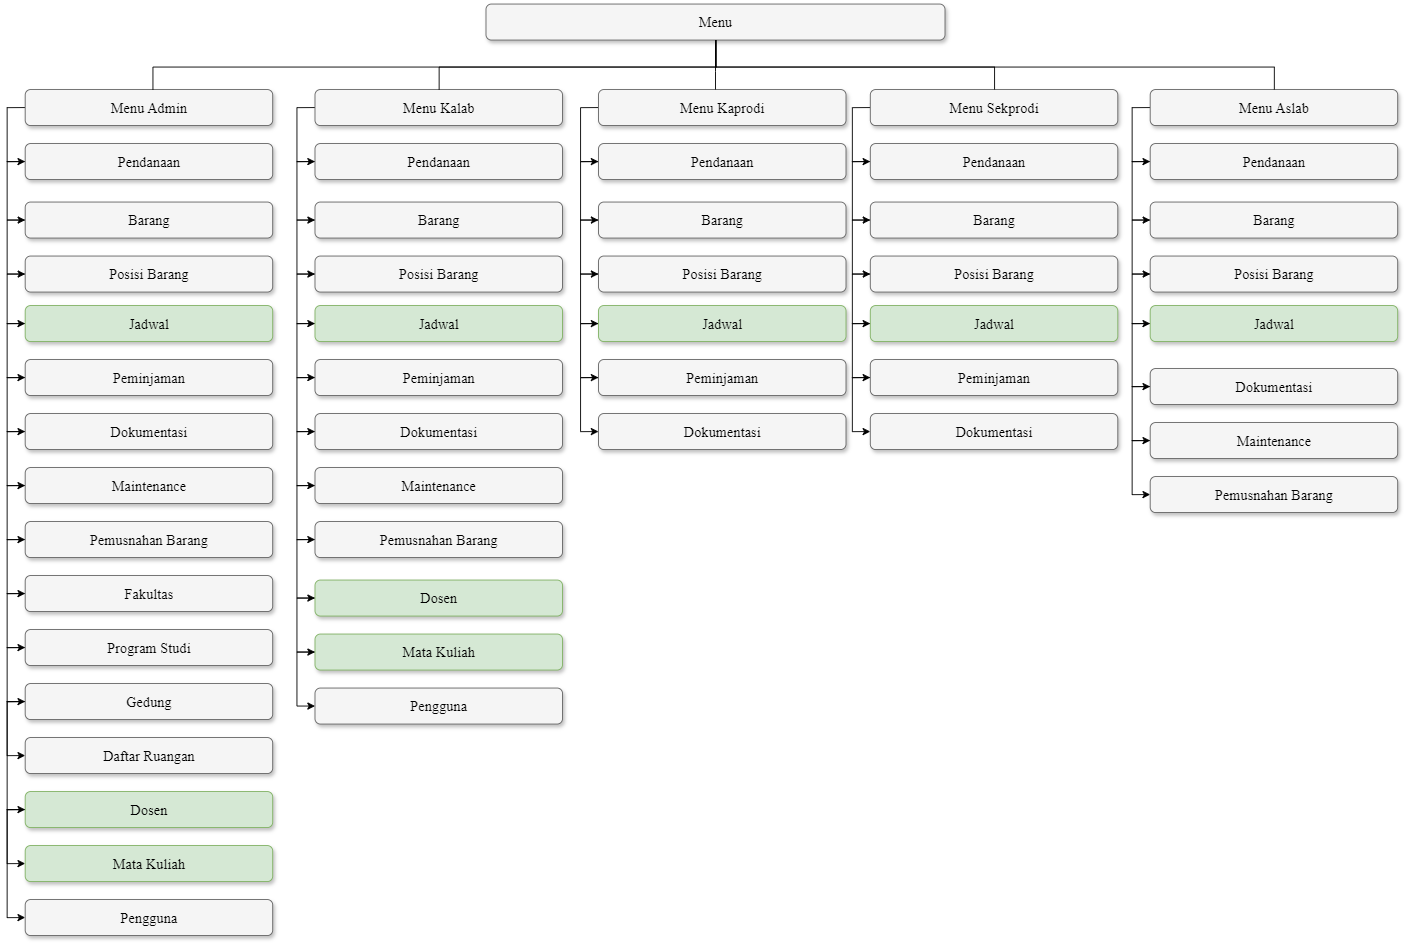
\includegraphics[width=1\textwidth]{konten/gambar/menu.png}
% 	\caption{Struktur Menu ILMIS}
% 	\label{StrukturMenuILMIS}
% \end{figure}

Pengembangan sistem ini menambahkan fitur baru yang ditandai dengan warna hijau pada struktur menu, termasuk fitur Jadwal untuk semua level pengguna (Admin, Kalab, Kaprodi, Sekprodi, dan Aslab) serta fitur Dosen dan Mata Kuliah yang kini dapat diakses oleh Kalab. Penambahan ini bertujuan untuk meningkatkan pengelolaan laboratorium dan efisiensi koordinasi antara pengelola dan dosen.

% =======================================================================================================================
\subsection{Perancangan \textit{Interface}}
Perancangan \textit{interface} berfungsi untuk menjelaskan tentang desain program sistem informasi manajemen laboratorium yang akan dibangun. Hal ini dilakukan untuk mempermudah pengguna dalam mengetahui proses yang terdapat pada sistem informasi manajemen laboratorium tersebut.

\begin{enumerate}
	\item Rancangan tampilan halaman utama yang berfungsi sebagai halaman pertama untuk sistem informasi manajemen laboratorium dapat dilihat pada Lampiran \ref{fig:landing-page-interface}.

	      {
	      \fontsize{10}{13}\selectfont
	      \begin{longtable}{p{4cm} p{9cm}}
		      \caption{Keterangan Tampilan Halaman Utama}                                                                                                                                                  \\
		      \hline
		      \textbf{Nomor \textit{Callouts}} & \textbf{Keterangan}                                                                                                                                       \\
		      \hline
		      \endfirsthead

		      \multicolumn{2}{c}{\normalsize\tablename\ \textbf{\thetable}\ {{Keterangan Tampilan Halaman Utama \space (Tabel lanjutan...)}}}                                                              \\
		      \hline
		      \textbf{Nomor \textit{Callouts}} & \textbf{Keterangan}                                                                                                                                       \\
		      \hline
		      \endhead

		      \hline
		      \endfoot

		      1                                & Browser toolbar dengan \texttt{width: 100\%}, \texttt{height: 40px}, \texttt{background-color: \#FFFFFF}                                                  \\
		      2                                & Logo berukuran \texttt{width: 40px}, \texttt{height: 40px}, dengan \texttt{margin-left: 24px} pada pojok kiri atas                                        \\
		      3                                & Navigation menu menggunakan \texttt{font-family: Poppins}, \texttt{font-size: 14px}, dengan \texttt{gap: 32px} antar menu                                 \\
		      4                                & Button Login dengan \texttt{padding: 8px 16px}, \texttt{border-radius: 6px}, \texttt{background-color: \#2563EB}                                          \\
		      5                                & Container header dengan \texttt{width: 100\%}, \texttt{height: 64px}, \texttt{box-shadow: 0 1px 3px rgba(0,0,0,0.1)}                                      \\
		      6                                & Text "Integrated Laboratory" menggunakan \texttt{font-family: Poppins}, \texttt{font-size: 48px}, \texttt{font-weight: 600}, \texttt{margin-bottom: 16px} \\
		      7                                & Text "Management Information System" berwarna \texttt{\#2563EB} dengan \texttt{font-weight: 600}                                                          \\
		      8                                & Button "Lihat Lebih Lanjut" dengan \texttt{padding: 12px 24px}, \texttt{background-color: \#2563EB}                                                       \\
		      9                                & Container image dengan \texttt{width: 560px}, \texttt{height: 400px}, \texttt{border-radius: 8px}                                                         \\
		      10                               & Container content dengan \texttt{max-width: 560px} dan \texttt{margin-right: 64px}                                                                        \\
		      11                               & Heading "Sistem Terintegrasi" dengan \texttt{text-align: center}, \texttt{font-size: 36px}, \texttt{margin: 64px 0 32px}                                  \\
		      12                               & Container cards dengan \texttt{display: grid}, \texttt{grid-template-columns: repeat(2, 1fr)}, \texttt{gap: 24px}                                         \\
		      13                               & Card pertama dengan \texttt{padding: 24px}, \texttt{background: white}, \texttt{border-radius: 8px}, \texttt{box-shadow: 0 1px 3px rgba(0,0,0,0.1)}       \\
		      14                               & Text content pada card dengan \texttt{font-size: 14px}, \texttt{line-height: 1.6}, \texttt{color: \#374151}                                               \\
		      15                               & Card kedua dengan styling sama seperti card pertama                                                                                                       \\
		      16                               & Card ketiga dengan styling sama seperti card pertama                                                                                                      \\
		      17                               & Section FAQ dengan \texttt{max-width: 800px}, \texttt{margin: 64px auto}                                                                                  \\
		      18                               & Container question dengan \texttt{padding: 24px}, \texttt{border-bottom: 1px solid \#E5E7EB}                                                              \\
		      19                               & Footer section dengan \texttt{background: \#1E293B}, \texttt{padding: 64px 24px}                                                                          \\
		      20                               & Footer links dengan \texttt{display: flex}, \texttt{gap: 32px}, \texttt{margin-top: 32px}                                                                 \\
		      21                               & Copyright text dengan \texttt{font-size: 14px}, \texttt{color: \#9CA3AF}                                                                                  \\
		      \hline
	      \end{longtable}
	      }

	\item Rancangan tampilan pilih aplikasi untuk login dapat dilihat pada Lampiran \ref{fig:pilih-login-interface}.


	      {

	      \fontsize{10}{13}\selectfont
	      \begin{longtable}{p{4cm} p{9cm}}
		      \caption{Keterangan Tampilan Halaman Selamat Datang}                                                                                     \\
		      \hline
		      \textbf{Nomor \textit{Callouts}} & \textbf{Keterangan}                                                                                   \\
		      \hline
		      \endfirsthead

		      \multicolumn{2}{c}{ \thetable\ {Keterangan Tampilan Halaman Selamat Datang} \space (Tabel lanjutan...)}                                  \\
		      \hline
		      \textbf{Nomor \textit{Callouts}} & \textbf{Keterangan}                                                                                   \\
		      \hline
		      \endhead

		      1                                & Text header "Selamat Datang" dengan \texttt{fonts Poppins}, warna font \texttt{\#73879C}              \\
		      2                                & Text sub-header "Silahkan pilih aplikasi yang akan anda gunakan" dengan \texttt{fonts Helvetica Neue} \\
		      3                                & Container card dengan \texttt{background color \#FFFFFF} dan \texttt{border-radius 8px}               \\
		      4                                & Link ILMIS dengan \texttt{icon users} dan text "Integrated Laboratory Management Information System"  \\
		      5                                & Link LABVIS dengan \texttt{icon users} dan text "Laboratory Visitor Information System"               \\
		      6                                & Link LARIS dengan \texttt{icon users} dan text "Laboratory Assistant Registration Information System" \\
		      \hline
	      \end{longtable}
	      }

	\item Rancangan tampilan kelola jadwal yang berfungsi untuk mengelola jadwal laboratorium dapat dilihat pada Lampiran \ref{fig:kelola-jadwal}. \selectfont


	      {
		      \fontsize{10}{13}\selectfont
		      \begin{longtable}{p{4cm} p{9cm}}
			      \caption{Keterangan Tampilan Kelola Jadwal}
			      \label{tab:ui-jadwal}                                                                                           \\
			      \hline
			      \textbf{Nomor \textit{Callouts}} & \textbf{Keterangan}                                                          \\
			      \hline
			      \endfirsthead
			      \multicolumn{2}{c}{\normalsize\tablename\ \textbf{\thetable}\ {Keterangan Tampilan Kelola Jadwal} \space (Tabel lanjutan...)}       \\
			      \hline
			      \textbf{Nomor \textit{Callouts}} & \textbf{Keterangan}                                                          \\
			      \hline
			      \endhead
						\hline
		      \endfoot

			      1                                & Button "Admin" dengan \texttt{icon arrow-right} di pojok kanan atas          \\
			      2                                & Text "Logout Aktif: Beranda / Jadwal" dengan \texttt{alignment right}        \\
			      3                                & Profile section dengan nama user "NIM: 1234567" dan foto profil              \\
			      4                                & Text header "Jadwal" dengan \texttt{fonts Helvetica Neue}                    \\
			      5                                & Button "Tambah Data" dengan warna \texttt{primary (\#2563EB)}                \\
			      6                                & Search input field dengan \texttt{icon search} di sebelah kanan              \\
			      7                                & Action buttons (\texttt{edit}, \texttt{delete}, \texttt{info}) di kolom Aksi \\
			      8                                & Data table dengan kolom: No, Hari/Tanggal, Jam, Ruangan, Aksi                \\
			      9                                & Sidebar menu dengan \texttt{icons} dan text untuk navigasi sistem            \\
			      \hline
		      \end{longtable}
	      }

	\item Rancangan tampilan tambah jadwal yang berfungsi untuk menambah jadwal laboratorium dapat dilihat pada Lampiran \ref{fig:tambah-jadwal-interface}.



	      {
	      \fontsize{10}{13}\selectfont
	      \begin{longtable}{p{4cm} p{9cm}}
		      \caption{Keterangan Tampilan Tambah Jadwal}
		      \label{tab:tambah-jadwal}                                                                                                                                                                                          \\
		      \hline
		      \textbf{Nomor \textit{Callouts}} & \textbf{Keterangan}                                                                                                                                                             \\
		      \hline
		      \endfirsthead

		      \multicolumn{2}{c}{\selectfont \thetable\ {Keterangan Tampilan Tambah Jadwal} \space (Tabel lanjutan...)}                                                                                                          \\
		      \hline
		      \textbf{Nomor \textit{Callouts}} & \textbf{Keterangan}                                                                                                                                                             \\
		      \hline
		      \endhead

		      1                                & Berisi menu navigasi dengan ikon dan teks, menggunakan \texttt{font-family: Poppins}, \texttt{font-size: 14px}. Memiliki warna latar gelap dan ikon menu terorganisir vertikal. \\
		      2                                & Field input untuk memasukkan tanggal dengan \texttt{placeholder dd/mm/yyyy}. Terdapat \texttt{ikon kalender} di sebelah kanan untuk membantu memilih tanggal.                   \\
		      3                                & Berisi beberapa form input untuk memasukkan data berikut:                                                                                                                       \\
		                                       & - Hari: Input teks untuk memilih atau memasukkan hari.                                                                                                                          \\
		                                       & - Jam Masuk dan Jam Keluar: Input waktu dengan \texttt{ikon jam} di sebelah kanan.                                                                                              \\
		                                       & - Nama Ruangan, Nama Mata Kuliah, dan Nama Dosen: \texttt{Dropdown} untuk memilih opsi.                                                                                         \\
		                                       & - Deskripsi: Area teks kosong untuk menambahkan keterangan lebih lanjut.                                                                                                        \\
		      4                                & Dua tombol aksi:                                                                                                                                                                \\
		                                       & - Tombol Kembali: Berwarna merah (\texttt{\#FF5A5F}) dengan \texttt{padding: 12px 24px}, \texttt{border-radius: 6px}.                                                           \\
		                                       & - Tombol Simpan: Berwarna biru (\texttt{\#2563EB}) dengan \texttt{padding: 12px 24px}, \texttt{border-radius: 6px}.                                                             \\
		      5                                & Teks di bagian bawah layar yang menampilkan informasi seperti hak cipta atau detail versi aplikasi. \texttt{Font-size} kecil dengan warna abu-abu muda.                         \\
		      \hline
	      \end{longtable}
	      }

	\item Rancangan tampilan edit jadwal yang berfungsi untuk mengedit jadwal laboratorium dapat dilihat pada Lampiran \ref{fig:edit-jadwal-interface}.

	      {
	      \fontsize{10}{13}\selectfont
	      \begin{longtable}{p{4cm} p{9cm}}
		      \caption{Tabel Keterangan Tampilan Edit Jadwal}
		      \label{tab:edit-jadwal}                                                                                                                                                                                            \\
		      \hline
		      \textbf{Nomor \textit{Callouts}} & \textbf{Keterangan}                                                                                                                                                             \\
		      \hline
		      \endfirsthead

		      \multicolumn{2}{c}{\selectfont \thetable\ {Tabel Keterangan Tampilan Edit Jadwal} \space (Tabel lanjutan...)}                                                                                                      \\
		      \hline
		      \textbf{Nomor \textit{Callouts}} & \textbf{Keterangan}                                                                                                                                                             \\
		      \hline
		      \endhead

		      1                                & Berisi menu navigasi dengan ikon dan teks, menggunakan \texttt{font-family: Poppins}, \texttt{font-size: 14px}. Memiliki warna latar gelap dan ikon menu terorganisir vertikal. \\
		      2                                & Field input untuk memasukkan tanggal dengan \texttt{placeholder dd/mm/yyyy}. Terdapat \texttt{ikon kalender} di sebelah kanan untuk membantu memilih tanggal.                   \\
		      3                                & Berisi beberapa form input untuk memasukkan data berikut:                                                                                                                       \\
		                                       & - Hari: Input teks untuk memilih atau memasukkan hari.                                                                                                                          \\
		                                       & - Jam Masuk dan Jam Keluar: Input waktu dengan \texttt{ikon jam} di sebelah kanan.                                                                                              \\
		                                       & - Nama Ruangan, Nama Mata Kuliah, dan Nama Dosen: \texttt{Dropdown} untuk memilih opsi.                                                                                         \\
		                                       & - Deskripsi: Area teks kosong untuk menambahkan keterangan lebih lanjut.                                                                                                        \\
		      4                                & Dua tombol aksi:                                                                                                                                                                \\
		                                       & - Tombol Kembali: Berwarna merah (\texttt{\#FF5A5F}) dengan \texttt{padding: 12px 24px}, \texttt{border-radius: 6px}.                                                           \\
		                                       & - Tombol Simpan: Berwarna biru (\texttt{\#2563EB}) dengan \texttt{padding: 12px 24px}, \texttt{border-radius: 6px}.                                                             \\
		      5                                & Teks di bagian bawah layar yang menampilkan informasi seperti hak cipta atau detail versi aplikasi. \texttt{Font-size} kecil dengan warna abu-abu muda.                         \\
		      \hline
	      \end{longtable}
	      }
\end{enumerate}
